
\subsection{CHIL Real-time Simulation Results}

As explained before, the objective for creating the proposed controller hardware-in-the-loop (CHIL) real-time simulation testbed, along with the respective API communication interfaces, is to create the means to rapidly prototype and validate any control system developed, in either Python or MATLAB, in a real-time environment. That is why, in order to verify the correct operation of the proposed testbed, the energy management system explained previously was integrated to the proposed testbed via the API functions developed, and a real-time CHIL test case was performed. For this case study, a 1-day test case was designed using the same conditions and parameters as the ones used in the offline verification, with the difference that all power system elements of the electrical power grid were modeled for real-time simulation as explained in Section \ref{SEC:TB}. Additionally,  the energy management controller agent was interfaced with the grid-connected DERs simulated inside the DRTS using the API functions and DNP3 communication as explained in Section \ref{SEC:API_DNM3}. 

\begin{figure}[!ht]
    \centering
    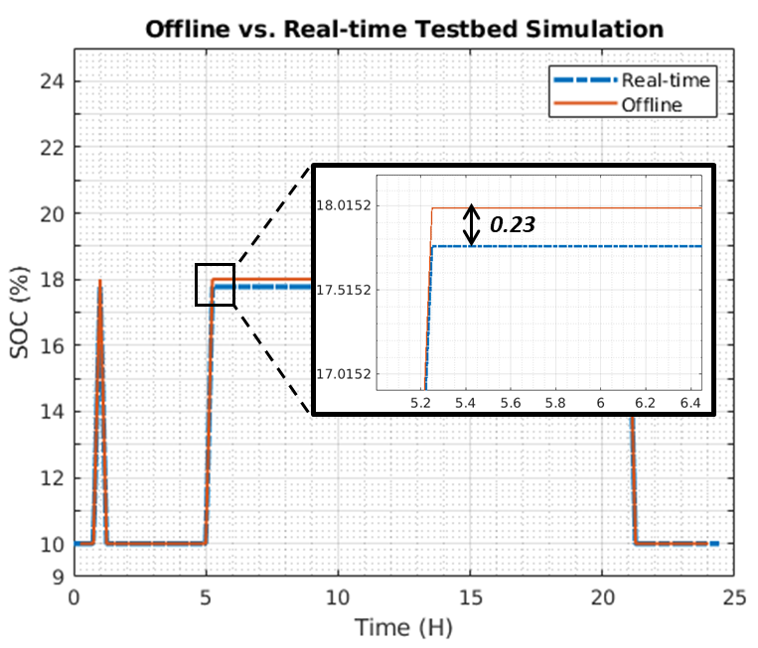
\includegraphics[width = 0.9\linewidth]{figs_juan/realtime_2.png}
    \caption{State-of-Charge reference for Energy Storage DER in 1-Day Real-time Controller Hardware-in-the-Loop (CHIL) test for Energy Management System.}
    \label{fig:realtime}
    \vspace{-1mm}
\end{figure}

Fig. \ref{fig:realtime} shows a comparison between the offline and real-time SOC values of the energy storage (ES). As observed, there are differences of around 0.23\%  in the SOC values obtained from the offline simulation test case when compared with the real-time CHIL test case. The differences between the offline and real-time simulation can be accounted to differences in the characteristics of the Lithium-ion ES, PV, and load models used in the offline Phasor simulation compared to the ones used in the real-time EMTP simulation. The usual round trip time for the communication was around 80 ms with a maximum round trip time of 2.09 seconds and the maximum time for computing a control action by the graph search algorithm was 4 seconds. Which means the controls took a maximum of 6.09 seconds to respond in the 24-hour long real-time simulation. The response time is more than adequate for the energy management solution running every 15 minutes (900 seconds). The proposed real-time CHIL testbed provides a more realistic picture of how an energy management system such as the one used here would operate in a real microgrid or distribution network setting. These realistic testing platform and resources have the capability of giving researchers a rapid way for testing state-of-the-art controllers designed to control grid-connected DERs in a real-time CHIL environment with a commonly used communication protocol, such as DNP3.


 
% \subsection{Communication Latency Tests for Real-time CHIL Testbed  Simulation Results}

% Several communications tests were performed with the objective of analyzing the latency and performance of the communication layer of the proposed CHIL testbed. These tests were performed using tools available in the RT-Lab DRTS software and double checked using an open-source packet analyzer called Wireshark. The DNP3 over TCP/IP packets were analyzed for integrity and latency tests inside Wireshark and their round-trip time (RTT) was recorded for a different number of values being sent and received. The main idea of these tests is to recognize the time it takes for a complete communication loop where states are sent from the DRTS to an external controller, and control actions are sent back from the controller. Fig. \ref{fig:wireshark_dnp3} shows the block diagram of the DNP3 communication between external controllers and the DRTS.


% \begin{figure}[t]
%     \centering
%     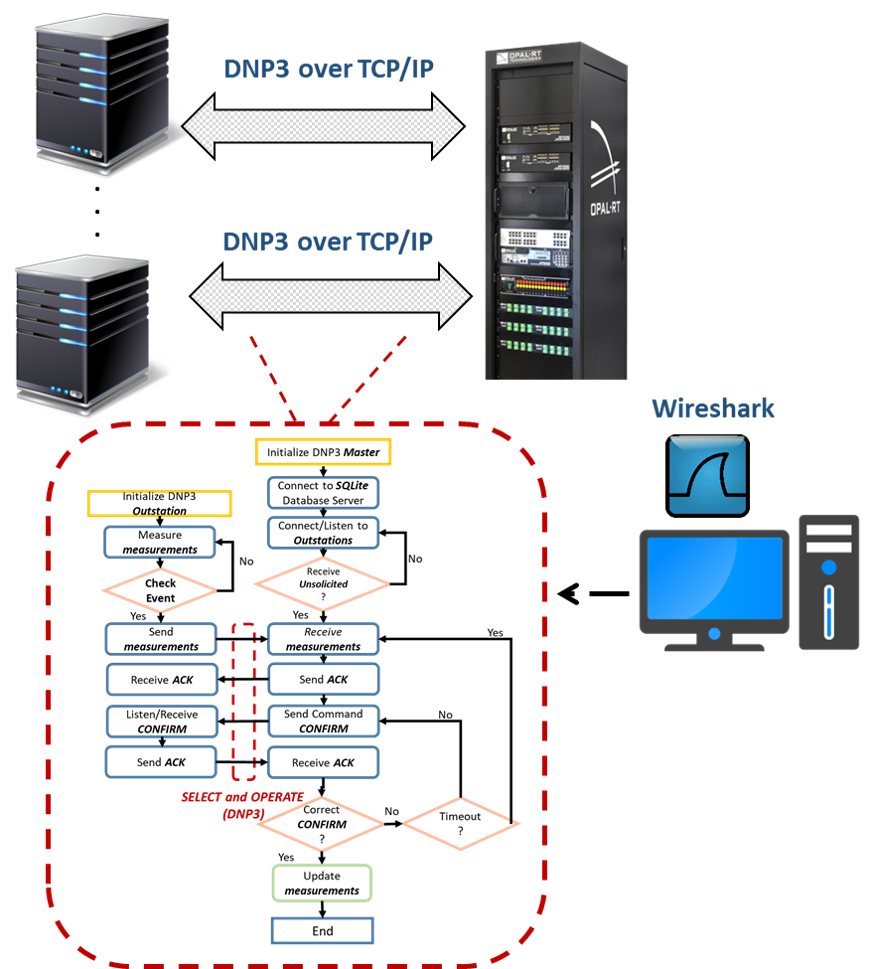
\includegraphics[width=8.5cm]{figs_juan/wireshark_dnp3.png}
%     \caption{Real-time Controller Hardware-in-the-Loop (CHIL) DNP3 Communication Latency Tests}
%     \label{fig:wireshark_dnp3}
% \end{figure}


% Table \ref{commtable} shows the specific timings or RTTs, recorded using the packet analyzer tools, and the average latency time for the communication tests. As observed in the results, as the number of values exchanged increases the communication latency increases. It is important to note that these tests assume that only one external controller is receiving and sending data to either multiple outstations or one outstation at a time, but if multiple external controllers are used, each with its own IP address and Port, then each controller would exhibit the same behavior seen in the proposed test case.


% \begin{table}[h!]
% \caption{DNP3 over TCP/IP Communication round-trip time (RTT) test results} % title of Table
% \begin{tabular}{|c|c|c|c|c|c|}
% \hline
% \textbf{\# of Values Exchanged} & \multicolumn{5}{c|}{\textbf{Round-Trip Time (s)}}                                                                                                                                              \\ \hline
% \multicolumn{1}{|l|}{}    & \multicolumn{1}{l|}{\textbf{Test 1}} & \multicolumn{1}{l|}{\textbf{Test 2}} & \multicolumn{1}{l|}{\textbf{Test 3}} & \multicolumn{1}{l|}{\textbf{Test 4}} & \multicolumn{1}{l|}{\textbf{Avg. RTT}} \\ \hline
% 3                         & 0.2748                               & 0.2504                               & 0.2896                               & 0.2654                               & \textbf{0.2701}                    \\ \hline
% 5                         & 0.4519                               & 0.4788                               & 0.4056                               & 0.4230                               & \textbf{0.4398}                    \\ \hline
% 10                        & 0.7451                               & 0.7245                               & 0.6995                               & 0.7793                               & \textbf{0.7371}                    \\ \hline
% 15                        & 1.0745                               & 1.1875                               & 1.1146                               & 1.1347                               & \textbf{1.1278}                    \\ \hline
% 20                        & 1.1218                               & 1.1922                               & 1.2906                               & 1.3004                               & \textbf{1.2262}                    \\ \hline
% 30                        & 2.1967                               & 2.2196                               & 2.0139                               & 1.9695                               & \textbf{2.0999}                    \\ \hline
% \end{tabular}
% \label{commtable} % is used to refer this table in the text
% \end{table}


% Additionally, as seen on the table, the timing delays observed are sufficient for applications with relatively large control time steps such as energy management applications and energy optimization controllers. It should be noted that the APIs and code implementation can be easily modified to support applications that require faster communication by changing the DNP3 configuration or using multiple controllers in parallel.





